\documentclass{article}
\usepackage[utf8]{inputenc}

\title{GET - Rapport- CandyFeine}
\author{Joel Schar, Yann Lederrey, Steve Henriquet, Anthoine Zaf }
\date{December 2018}

\usepackage{natbib}
\usepackage{graphicx}

\begin{document}

\maketitle

\section{Introduction}
> quel problématique notre produit va-t-il résoudre <

\section{Business Modèle}

\section{Structure juridique}
Nous choisissons de faire une Société à responsabilité limitée (Sarl)
Cela car nous serions un petite entreprise et que le capital initial est raisonnable : 20 milles CHF.

\section{Diagnostic stratégique de votre activité}

\section{Publique Cible}
Le bonbon "CandyFein" est un bonbon qui se veut énergisant. Il sera consommé au ressenti d'une baisse d'energie ou d'un besoin d'attention accrue. En début de jounrée, après un bon repas, en fin de journée ou début de soirée ce tout des petit moment ou un petit coup de fouet avant de repartir peut s'avérer nécessaire.\\
Ce type de besoin est plutôt typique d'une population active qui à une journée bien remplie. Un publique jeune qui ne veut pas forcément prendre le temps de s'arrêter pour boire un café et qui préfère gagner du temps en mangeant une petite dose d'énergie, délicieusement sucrée, en même temps qu'il fait autre chose.\\
Ce produit parfaitement dosé saura trouver sa place dans la poche d'un blouson et sera facilement accessible en tout temps.\\

\section{Le Produit}
CandyFeine
\subsection{Caractéristiques du produit}
CandyFeine sont des bonbons pétillants gelifiés en forme de grains de café comprenant de la cafeine et à de différents gouts.
Vendu sous forme de paquets de 10 ou 20 bonbons.
\subsection{Assortiment, gamme}
\textbf{Différents gout de bonbons :}

\textit{* : signifie que c'est encore en prototype}
\begin{itemize}
 \item Pomme-citron avec sucre pétillant
 \item Citron avec sucre pétillant
 \item framboise avec sucre pétillant
 \item café *
\end{itemize}

\textbf{Différents produits energisant :}
\begin{itemize}
 \item Caféine
 \item Guarana *
\end{itemize}

\subsection{Ingrédients}
\textbf{Correspond à la préparation de 180 grammes de bonbons pétillant pomme-citron}
\textbf{ingérdients des bonbons}

\textit{Certaines recettes peuvent contenir du colorant alimentaire naturels}
\begin{itemize}
 \item 100ml de jus de pomme
 \item 100g de sirop de glucide
 \item 8g d'amidion
 \item 8g d'agar agar
 \item 4g d'extrait de citron
 \item 135mg de caféine pure
\end{itemize}

\textbf{ingrédients du sucre acidulé}
\begin{itemize}
 \item 6g d'acide citrique
 \item 18g de sucre fin
\end{itemize}

\subsection{Qualité}
Produit de manière artisanale dans le respect des fournisseurs et des consommateur.
CandyFeine joue sur la transparence de ses produits et leur provenance.
Nous assurons des produits de qualité, le plus local possible. Nos bonbons sont vegans.
\subsection{Marque}
Au sein de l'entreprise CandyFeine Sàrl notre marque CandyFeine décrit le produit en un mot, candy pour le bonbon et Feine en rapport à la cafeine contenue à l'intérieur.
Le nom de la marque permet donc de rapidement assimiler le nom à un type de produit et l'anglisisme permet plus facielement l'exportation des bonbons.

\subsection{Accessoires}
Dans l'état actuelle des choses nous n'avons pas jugé utiles la création d'accessoires.

\subsection{Packaging}
Actuellement nous proposons nos bonbons par paquet de 10 ou 20, Ceci correspond à la dose d'une ou deux boisson energisantes connue du marché actuel.
Le packaging est sous-forme de sachet avec une étiquette décrivant les ingrédients des bonbons.

\begin{figure}[H]
\centering
   \caption{\label{étiquette} étiquette des CandyFeine gout café}
   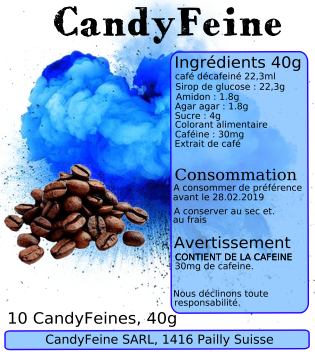
\includegraphics[scale=1]{../img/designEtiquettes_Cafe.png}

   \caption{\label{étiquette} étiquette des CandyFeine gout citron}
   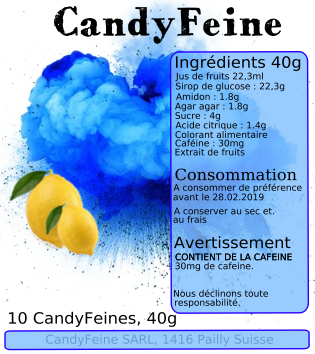
\includegraphics[scale=1]{../img/designEtiquettes_Citron.png}
\end{figure}
\begin{figure}[H]
\centering
   \caption{\label{étiquette} étiquette des CandyFeine gout framboise}
   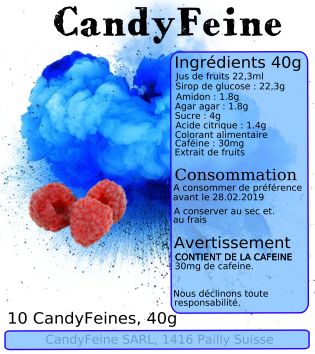
\includegraphics[scale=1]{../img/designEtiquettes_Framboise.png}

   \caption{\label{étiquette} étiquette des CandyFeine gout pomme-citron}
   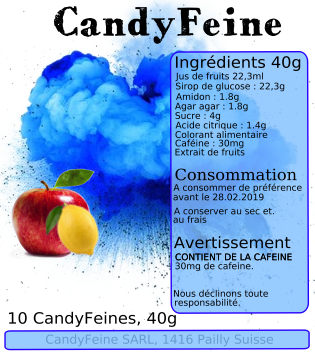
\includegraphics[scale=1]{../img/designEtiquettes_pommeCitron.png}

\end{figure}


\subsection{Prestations annexes}
A l'heure actuelle nous proposants uniquement le conseil client comme préstation annexe.

\section{Modèle du Produit}

\section{Processus}
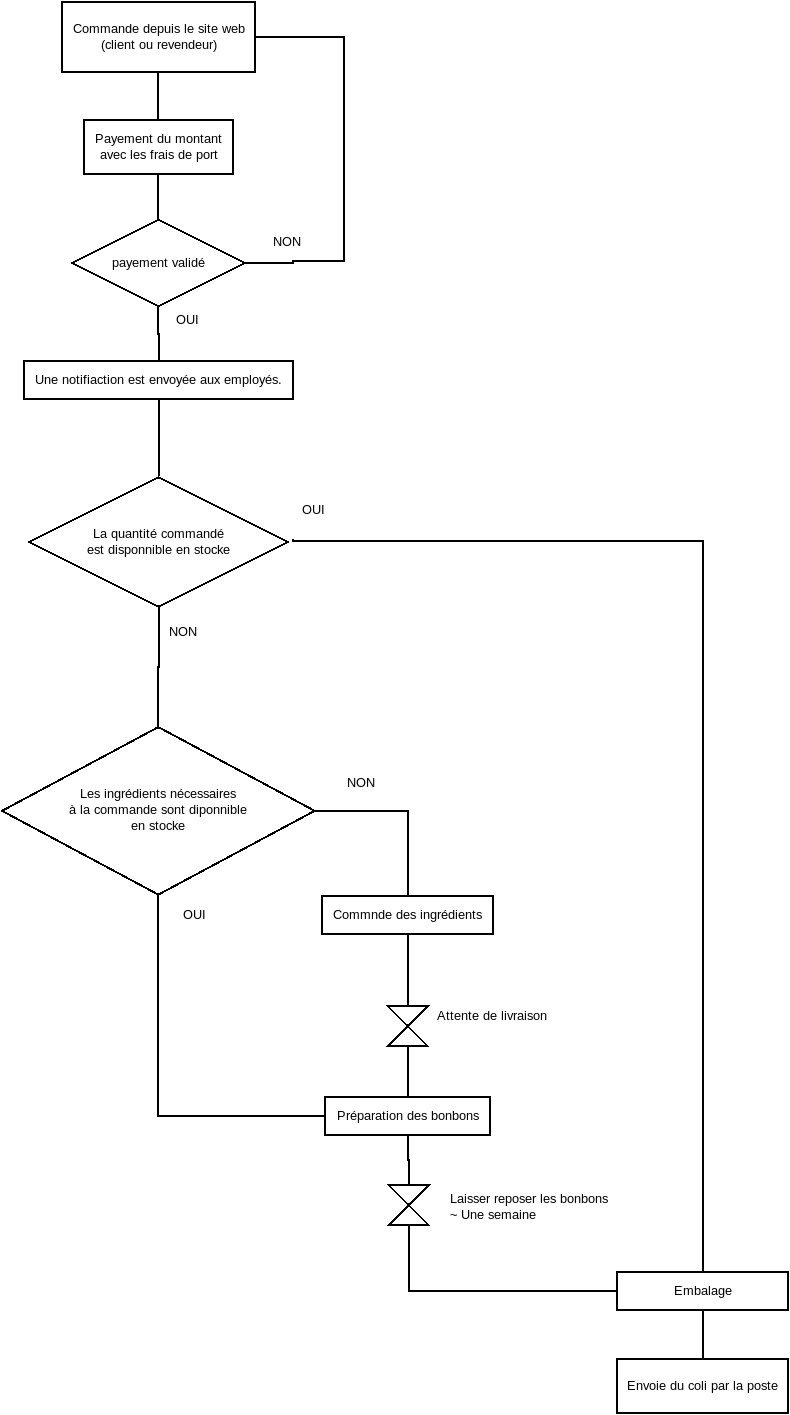
\includegraphics[scale=0.4]{../processus_de_commande.png} 

\section{Prix}
Ingrédients ( matière première ) : 0.35 CHF \\
Prix final du produit :  4.50 CHF\\

Cette différence de prix nous permet de couvrir les frais de production, d'amortir l'investissement et de dégager un salaire correct pour les employés et le travail fourni.

\section{Objectifs commerciaux}
\subsection{Stratégie d'attirance des clients}
Notre produits peut toucher un vaste pannel de personne nous pouvons tout de meme
nous centrer sur le monde étudiants qui sont de grand consommateurs de caféine, ainsi que les conducteurs ou encore des sportifs.\\
L'idée est donc de faire de commencer la publicité auprès des université et des stations services. Par la suite on peu immaginer aller à des
foir ou passer sur de la publicité de plus grande échelle tel que radio, affiches publicitaires.
\subsection{preuves de traction}
Actuellement seul le monde estudiantin a été interpellé par rapport à notre produit. Ces derniers se trouvent etre intéressé par son apport en caféine.
\subsection{cout d'qcquisition des clients}
Dans le cas ou on commence la publicité par l'approche des étudiants et de stations services, il faut compter le cout en trajet, en affiche A4 publicitaire ainsi qu'en rabais sur les bonbons afin d'attirer les clients.

\subsection{expension du nombre de clients}
Par la suite, il faudrait réussir à faire notre place face aux produits energétiques existants. Pour cela le bouche à oreille et le buzz est notre plus grande chance.\\
En cas de buzz, on peut donc imaginer une augmantation rapide et exponentielle du nombre d'acheteurs.\\
Dans l'autre cas, il faudrait voir une augmantation plus stable et lent des consommateurs.

\section{Publicité}

\section{Budget prévisionnel sur 3-5 ans}

\section{Conclusion}

\bibliographystyle{plain}
\bibliography{références}
\end{document}
